\def\problemset#1#2#3{
\noindent\rule{16.5cm}{1pt}
\begin{center}
  \parbox{16.5cm}{\bf
    STAT 598Z Homework 3 \\
    Instructor: Prof. S V N Vishwanathan \hfill Jiajie Huang\\
    Due Feb 26th, 2013 \hfill huang147@purdue.edu
    }
\end{center}
\noindent\rule{16.5cm}{0.5pt}
}

\newcommand{\lb}[1]{\left \lfloor #1 \right \rfloor}
\newcommand{\bmat}[1]{\begin{bmatrix} #1 \end{bmatrix}}
\documentclass[fleqn, 11pt]{article}
\usepackage{fullpage}
\usepackage{hyperref}
\usepackage{ulem}
\usepackage{amsmath}
\usepackage{algorithm}
%\usepackage{algorithmic}
\usepackage{algpseudocode}
\setlength{\parindent}{0in}
\usepackage{graphics}
\usepackage{graphicx}
\usepackage{mathtools}


\begin{document}

\problemset{3}{Problem Set 2}{\today}


\section*{Problem 1}
For this problem, I first do a quicksort on the list, then find out the median, which is the number indexed as $\frac{n+1}{2}$ ($n$ is odd) or the average of the two numbers indexed as $\frac{n}{2}$ and $\frac{n}{2} + 1$ ($n$ is even). See my code below: 

\begin{verbatim}

import numpy as np
import numpy.random as rand

# Given a list of unsorted numbers, this program first sorted it, then find the median

# define a quicksort function to sort a list
def sort(a):
    n = len(a)
    if n <= 1:
        return a
    else:
        pivotIndex = int(n/2)
        pivot = a[pivotIndex]
        large = []
        small = []
        a.remove(pivot)
        for i in range(n-1):
            if a[i] <= pivot:
                small.append(a[i])
            else:
                large.append(a[i])
        a = sort(small) + [pivot] + sort(large)
        return a


# define a function to find median from a sorted list
def medianFromSorted(a):
    n = len(a)
    if n == 0:
        print "array can not be empty!"
    elif n == 1:
        median = a[0]
    else:
        if n%2:
            median=a[n/2]
        else:
            median = float(a[n/2]+a[n/2-1])/2
    return median


# get median from a list (no matter sorted or not)
def median(a):
    a = sort(a)
    median = medianFromSorted(a)
    return median


# Test on several different lists to ensure correctness

b = [1,2,3,4,4,5]
print "before sort:", b
b = sort(b)
print "after sort:", b
print "median:", median(b)

b = [1,7,12,4,3,2,5]
print "before sort:",b
b = sort(b)
print "after sort:",b
print "median:", median(b)

# generate list b of random numbers
b = []
for i in xrange(10):
    v = rand.randint(100)
    b.append(v)
print "before sort:", b
b = sort(b)
print "after sort:", b
print "median:", median(b)

\end{verbatim}


The recursion tree for quicksort is shown in Figure \ref{recursion}. \\

\begin{figure}[htb]
\centering
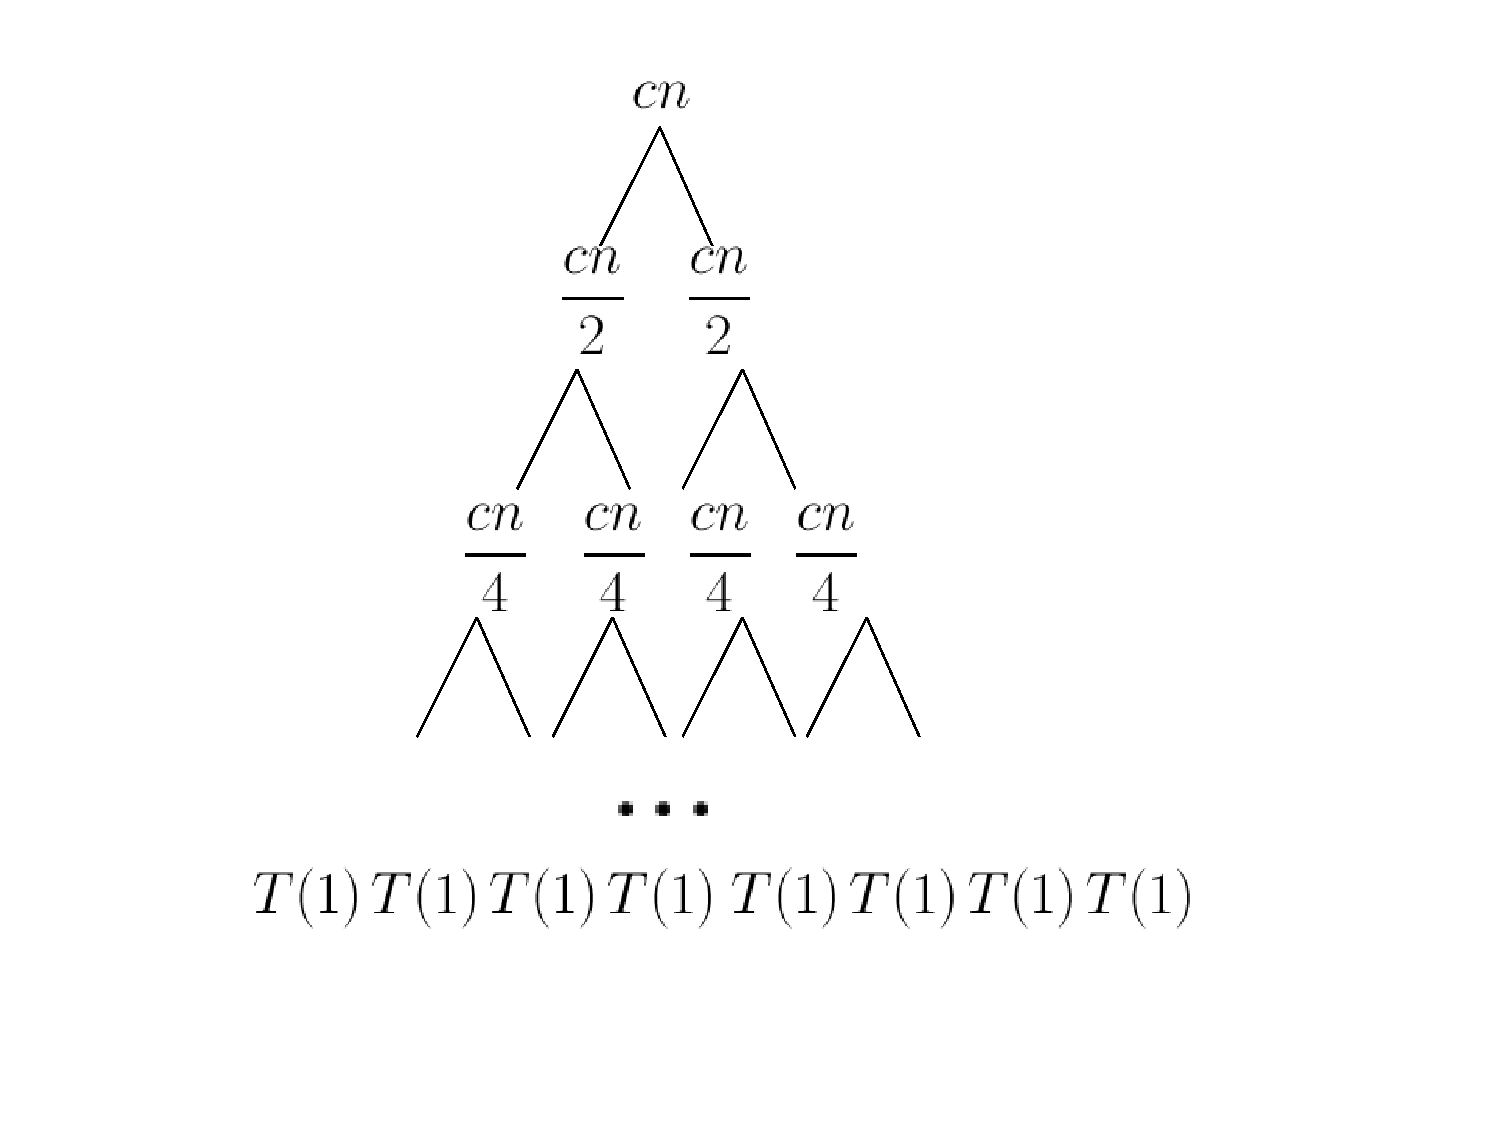
\includegraphics[width=10cm]{hw3p1fig.pdf}
\caption{Recursion Tree for Quicksort}
\label{recursion}
\end{figure}



Thus, for quicksort, we have 
\[
T(n) = 2 T(\frac{n}{2}) + cn = 2 ( 2 T(\frac{n}{4}) + c \frac{n}{2} ) + cn = 2^2 T(\frac{n}{2^2}) + 2cn = ... = 2^k T(\frac{n}{2^k}) + kcn = 2^k T(1) + kcn
\]

In the end, we have $k$ levels in the recursion tree, and $2^k = n$, so $k = log_2{(n)}$. The equation becomes 
\[
T(n) = n T(1) + cnlog_2{(n)} = O(nlog_2{(n)})
\]

Considering the time complexity got from getting the median, which is $0$ ( $n$ is odd) or $2$ ($n$ is even) basic operations, definitely, our total time complexity is bound at $O(nlog_2{(n)})$.


\section*{Problem 2}

\begin{itemize}

\item Create numpy array x and print x
\begin{verbatim}
import numpy as np

x = np.arange(1,16)
print "x:", x
\end{verbatim}

\item Reshape x into 5*3 matrix A and print A
\begin{verbatim}
A = x.reshape(5,3)
print "A:", A
\end{verbatim}

\item Extract row 1,2,4 and column 1,3 to make a matrix B and print B. Also multiply B by vector (5,3) and print the result
\begin{verbatim}
# take row 1,2,4 and column 1,3 and make matrix B; print B
B = (A[(0,1,3),:])[:,(0,2)]
print "B:", B
# make a vector (3,5)
y = np.array([[3],[5]])
# multiply B by the vector (3,5) and print the result
By = np.dot(B, y)
print "By:", By
\end{verbatim}

\item Reshape x into 5 * 3 matrix C and print C
\begin{verbatim}
C = (x.reshape(3,5)).T
print "C:", C
\end{verbatim}

\end{itemize}


\section*{Problem 3}
In this problem I generate a $4-D$ array from standard normal distribution (i.e. Gaussian distribution with mean = $0$ and std = $1$) with $(4,3,8,6)$ as its four dimensions. The $numpy$ functions $numpy.random.standard\_normal$ will give me the random numbers from standard normal; $numpy.mean$, $numpy.std$, $numpy.var$, $numpy.max$, and $numpy.min$ will give me the corresponding statistics for the array no matter how many dimensions it has. \\
 
See my code below: 

\begin{verbatim}
import numpy as np
import numpy.random as rand

# generate random numbers from standard normal distribution
# standard normal = Gaussian with mean = 0 and std = 1
# first seed the random number generator
rand.seed(201314)
size = 4 * 3 * 8 * 6
a = np.array(rand.standard_normal(size))
# resize a so it has shape (4,3,8,6)
a.resize(4,3,8,6)

# find the mean, std, var, min, max for a
print "mean(a):", np.mean(a)
print "std(a):", np.std(a)
print "var(a):", np.var(a)
print "min(a):", np.min(a)
print "max(a):", np.max(a)
\end{verbatim} 


The output using my code, for which the mean and std are close to those in a standard normal distribution:
\begin{verbatim}
mean(a): 0.0518500555208
std(a): 0.979626554723
var(a): 0.959668186718
min(a): -2.94328259078
max(a): 3.23038575557
\end{verbatim}


\section*{Problem 4}
In this problem, I generate $1000$ evenly spaced numbers from the given interval $[-10,10]$ to make a numpy array $x$, then produce the plot of $f(x)$ vs $x$. I also used $optimize.fmin\_bfgs$ from scipy package to find the minimum of $f(x)$. The plot in Figure \ref{fmin} shows that, the minimum visible on the plot agrees with the output of $optimize.fmin\_bfgs$ shown below: 
\begin{verbatim}
Value of x when f(x) is minimized: [-0.62644628] 
Minimum value of f(x): [2.35476044]
\end{verbatim}

\begin{figure}[htb]
\centering
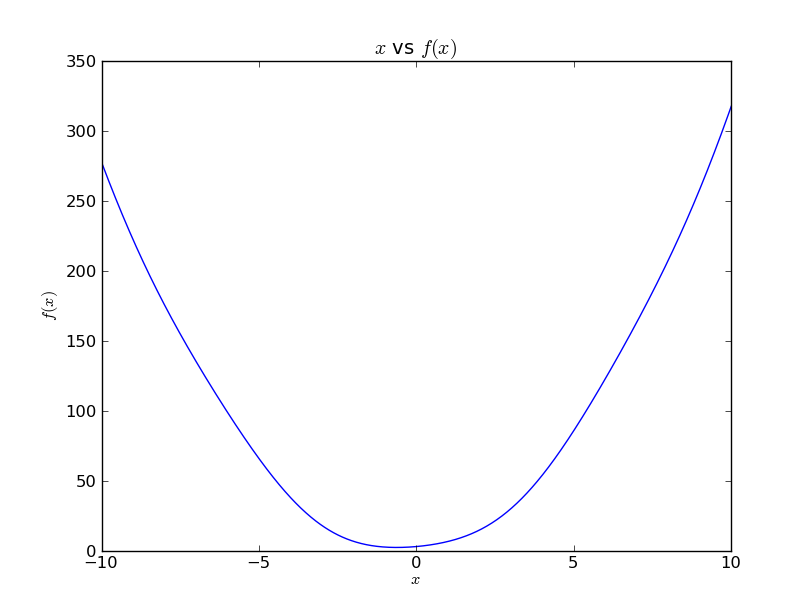
\includegraphics[width=15cm]{hw3p4.png}
\caption{Plot of $f(x)$ vs $x$}
\label{fmin}
\end{figure}


See my code below:

\begin{verbatim}
import numpy as np
import matplotlib.pyplot as plt
from scipy import optimize

# defined the function
def fx(x):
    return 2*x + 3*x**2 + 3*np.cos(x)

# gradient of the function
def grad_fx(x):
    return 2 + 6*x - 3*np.sin(x)

# initialize x and y as two list of numbers
x = np.linspace(-10,10,num = 1000)
y = []

# give an intial value for x
x0 = 1

# do the optimization and print the result
xopt = optimize.fmin_bfgs(fx, x0, fprime=fx)
print "Value of x when f(x) is minimized:", xopt, "Minimum value of f(x):", fx(xopt)

# get the values of y = f(x) by calculation
for i, v in enumerate(x):
    y.append( fx(v) )

# make the plot
plt.plot(x,y)
plt.title(r"$x$ vs $f(x)$")
plt.xlabel(r"$x$")
plt.ylabel(r"$f(x)$")
plt.show()

\end{verbatim}


\section*{Problem 5}
The plot is shown in Figure \ref{tri} below. I want to point out that in the third subplot of $tan(x)$ vs $x$, since the limit of $y$ is $[-1,1]$, the $y$ values outside of this limit is not shown in the plot here. \\

\begin{figure}[htb]
\centering
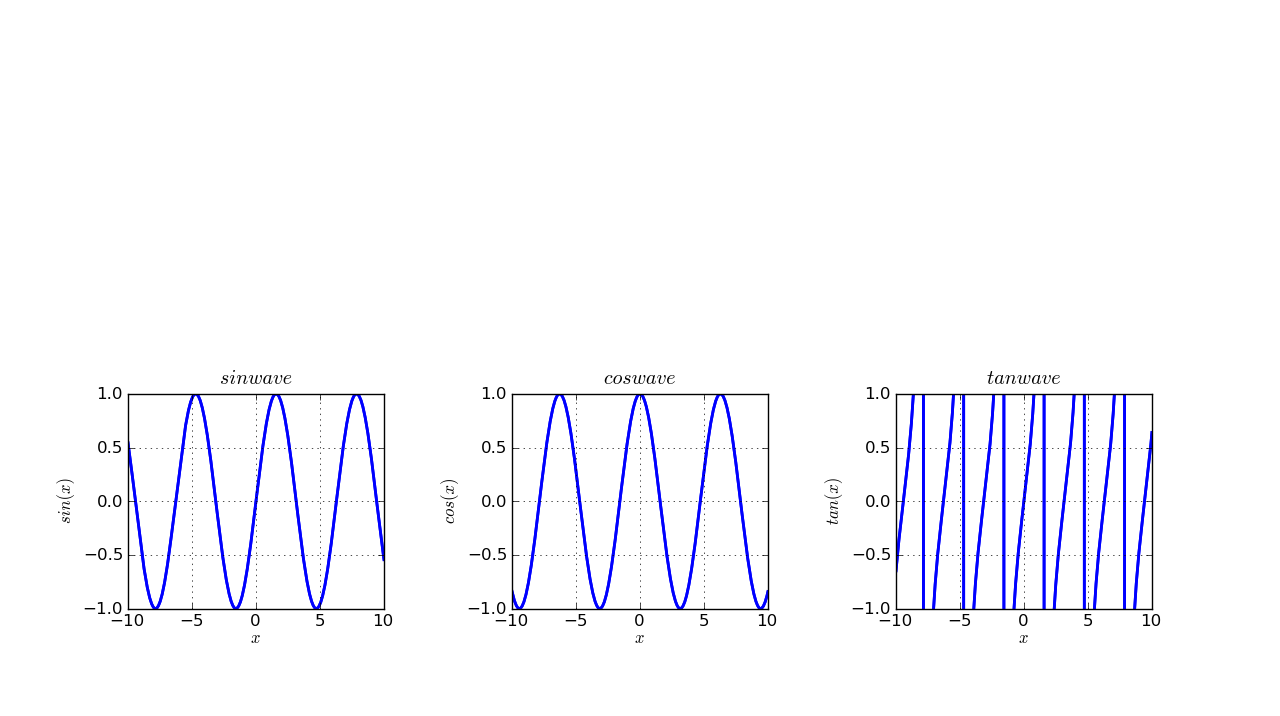
\includegraphics[width=18cm]{triangular.png}
\caption{Plot of $sin(x)$ vs $x$, $cos(x)$ vs $x$, and $tan(x)$ vs $x$}
\label{tri}
\end{figure}

See my code below: 
\begin{verbatim}
import numpy as np
import matplotlib.pyplot as plt

# define 3 functions
def fx(x):
    return np.sin(x)

def gx(x):
    return np.cos(x)

def hx(x):
    return np.tan(x)

# limit x on interval [-10,10]
x = np.linspace(-10,10,num = 10000)

# get the y on different functions
yf = []
yg = []
yh = []

for v in x:
    yf.append(fx(v))
    yg.append(gx(v))
    yh.append(hx(v))


# make the plots for f(x), g(x), and h(x)
# set figure size and resolution
fig = plt.figure(1,figsize = (15,10),dpi=100)
# the first subplot: f(x) vs x
pyf = fig.add_subplot(1,3,1)
# make the plot, specify line color and width
pyf.plot(x,yf,'b',linewidth=2)
# set the position of subplot so it won't overlap with other subplots
pyf.set_position([0.10,0.15,0.20,0.30])
# plot the grid
plt.grid(True)
# limit y value on interval [-1,1]
plt.ylim(-1,1)
# plot title and x, y labels
plt.title(r"$sin wave$")
plt.xlabel(r"$x$")
plt.ylabel(r"$sin(x)$")


pyg = fig.add_subplot(1,3,2)
pyg.plot(x,yg,'b',linewidth=2)
pyg.set_position([0.40,0.15,0.20,0.30])
plt.grid(True)
plt.ylim(-1,1)
plt.title(r"$cos wave$")
plt.xlabel(r"$x$")
plt.ylabel(r"$cos(x)$")


pyh = fig.add_subplot(1,3,3)
pyh.plot(x,yh,'b',linewidth=2)
pyh.set_position([0.70,0.15,0.20,0.30])
plt.grid(True)
# set the limit of y to be [-1,1]
# please note that y here has a lot more value points outside this limit
plt.ylim(-1,1)
plt.title(r"$tan wave$")
plt.xlabel(r"$x$")
plt.ylabel(r"$tan(x)$")


# save figure and show it on screen
fig.savefig('triangular.png')
plt.show()
                  
\end{verbatim}

\end{document}